\documentclass[tikz,border=10pt]{standalone}
\begin{document}
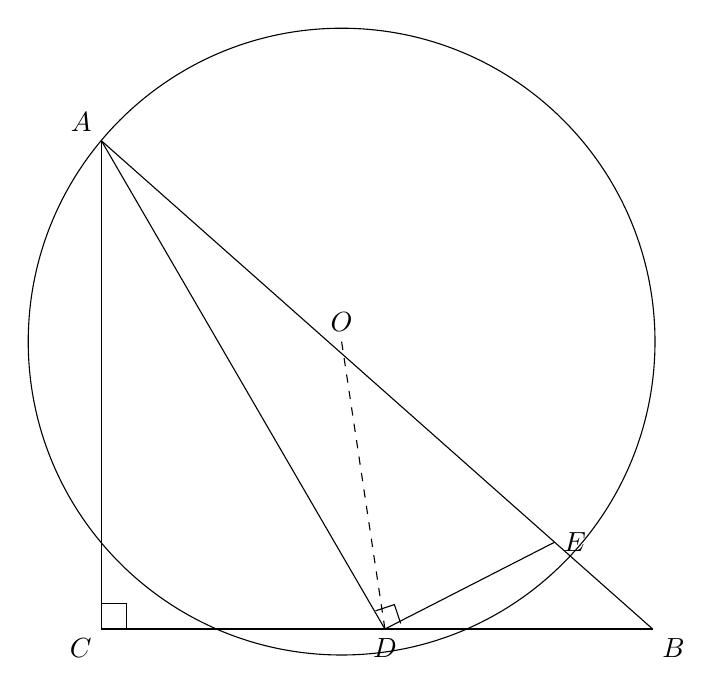
\begin{tikzpicture}[scale=1]

% Coordinates
\coordinate (C) at (0,0);
\coordinate (B) at (7,0);
\coordinate (D) at (3.6,0);
\coordinate (A) at (0,6.2);
\coordinate (O) at (3.05,3.65);
\coordinate (E) at (5.75,1.1);

% Baseline and main segments
\draw (C) -- (B);
\draw (A) -- (C);
\draw (A) -- (D);
\draw (A) -- (B);
\draw (D) -- (E);
\draw[dashed] (O) -- (D);

% Circle
\draw (O) circle[radius=3.98];

% Right-angle mark at C
\draw (0,0.32) -- (0.32,0.32) -- (0.32,0);

% Right-angle mark at D between AD and DE
\draw (3.48,0.23) -- (3.72,0.31) -- (3.80,0.07);

% Labels
\node[above left] at (A) {$A$};
\node[below left] at (C) {$C$};
\node[below right] at (B) {$B$};
\node[below] at (D) {$D$};
\node[above] at (O) {$O$};
\node[right] at (E) {$E$};

\end{tikzpicture}
\end{document}
